\documentclass[a4paper,12pt]{article}

\usepackage[utf8]{inputenc}
\usepackage[T1]{fontenc}
\usepackage[brazil]{babel}
\usepackage{graphicx}
\usepackage{amsmath}
\usepackage{float}
\usepackage{geometry}
\usepackage{hyperref}
\usepackage{array}
\usepackage{booktabs}
\usepackage{longtable}
\usepackage{caption}
\usepackage[numbers]{natbib}

\geometry{margin=2.5cm}

\hypersetup{
    colorlinks=true,
    linkcolor=black,
    urlcolor=blue,
    citecolor=black
}

\begin{document}

%====================================================
% CAPA
%====================================================

\begin{titlepage}
    \centering

    
\includegraphics[width=0.22\textwidth]{ufla-logo.png}

    \vspace{1cm}

    {\Large \textbf{UNIVERSIDADE FEDERAL DE LAVRAS}}\\[0.3cm]
    {\large PROGRAMA DE PÓS-GRADUAÇÃO EM ENGENHARIA DE SISTEMAS E AUTOMAÇÃO}\\[2cm]

    {\Large \textbf{COMPUTAÇÃO EVOLUCIONÁRIA}}\\[1cm]

    {\LARGE \textbf{Implementação do Algoritmo Genético}}\\[2cm]

    \begin{flushleft}
    \textbf{Discentes:}\\
    Matheus Higino\\
    Marcos Vinicius Cardoso Reis\\[0.8cm]

    \textbf{Professor:}\\
    Bruno Henrique Groenner Barbosa
    \end{flushleft}

    \vfill

    {\large Lavras -- MG}\\
    {\large Abril de 2026}

\end{titlepage}

%====================================================
% SUMÁRIO
%====================================================

\tableofcontents
\newpage

%====================================================
% INTRODUÇÃO
%====================================================

\section{Introdução}

Os Algoritmos Genéticos (AGs) são técnicas de otimização inspiradas no processo de evolução natural e pertencem ao grupo dos algoritmos evolutivos. Seu funcionamento baseia-se em operadores como seleção, recombinação e mutação, simulando o processo evolutivo biológico com o objetivo de encontrar soluções ótimas ou próximas do ótimo global \cite{goldberg1989}.

Essa abordagem foi amplamente consolidada na literatura como uma das principais estratégias para resolução de problemas complexos de busca e otimização, especialmente em cenários com múltiplos ótimos locais e espaços de busca extensos \cite{mitchell1998}. Sua principal vantagem está na capacidade de explorar diferentes regiões do espaço de soluções simultaneamente, reduzindo a dependência de condições iniciais específicas.

Neste trabalho foi implementado um Algoritmo Genético simples para a resolução de dois problemas de otimização com duas variáveis, conforme solicitado na disciplina de Computação Evolucionária. A implementação contemplou representação cromossomial binária, seleção por roleta viciada e torneio, cruzamento com um ponto de corte por variável, mutação bit a bit e elitismo opcional.

Além da implementação do algoritmo, foram realizados experimentos com diferentes combinações de parâmetros, incluindo probabilidade de cruzamento, probabilidade de mutação, método de seleção, tamanho da população, número de gerações, uso de elitismo e função objetivo. Para cada configuração, foram executadas 30 repetições, permitindo uma análise estatística mais robusta dos resultados obtidos.

%====================================================
% METODOLOGIA
%====================================================

\section{Metodologia}

\subsection{Representação Cromossomial}

Cada indivíduo foi representado por um cromossomo binário de 32 bits, dividido em duas partes:

\begin{itemize}
    \item 16 bits para representar a variável $x$;
    \item 16 bits para representar a variável $y$.
\end{itemize}

Após a codificação binária, os valores foram convertidos para números reais no intervalo $[-10,10]$, possibilitando a avaliação das funções objetivo.

\subsection{Problemas de Otimização}

Foram escolhidas duas funções clássicas da literatura de otimização contínua, ambas com duas variáveis e características multimodais.

\subsubsection{Cross-in-Tray}

\begin{equation}
f(x,y) =
-0.0001
\left(
\left|
\sin(x)\sin(y)
\exp\left(
\left|
100 - \frac{\sqrt{x^2 + y^2}}{\pi}
\right|
\right)
\right|
+ 1
\right)^{0.1}
\end{equation}

A função Cross-in-Tray é conhecida por apresentar grande quantidade de ótimos locais, o que a torna particularmente desafiadora para algoritmos de busca.

\subsubsection{Drop-Wave}

\begin{equation}
f(x,y) =
-
\frac{
1 + \cos(12\sqrt{x^2 + y^2})
}{
0.5(x^2 + y^2) + 2
}
\end{equation}

A função Drop-Wave também é multimodal, porém tende a apresentar comportamento mais regular do que a Cross-in-Tray.

Como o Algoritmo Genético foi estruturado como um problema de maximização de fitness, foi necessário adaptar as funções objetivo de forma adequada para esse contexto.

\subsection{Operadores Genéticos}

Foram implementados os seguintes operadores:

\begin{itemize}
    \item \textbf{Seleção por roleta viciada}: baseada na probabilidade proporcional ao fitness;
    \item \textbf{Seleção por torneio}: seleção do melhor indivíduo entre um subconjunto aleatório;
    \item \textbf{Cruzamento}: um ponto de corte para cada variável;
    \item \textbf{Mutação}: bit a bit;
    \item \textbf{Elitismo}: opcional, permitindo preservar o melhor indivíduo de cada geração.
\end{itemize}

Durante o desenvolvimento, verificou-se a necessidade de normalizar os valores de fitness na seleção por roleta, uma vez que a utilização de valores negativos provocava falhas no processo de seleção probabilística. Esse ajuste foi importante para garantir o funcionamento correto do algoritmo.

\subsection{Configurações Avaliadas}

Foram avaliadas combinações dos seguintes parâmetros:

\begin{itemize}
    \item Probabilidade de cruzamento: 0.6, 0.8 e 1.0;
    \item Probabilidade de mutação: 0.01, 0.05 e 0.1;
    \item Método de seleção: roleta e torneio;
    \item Tamanho da população: 20, 50 e 100;
    \item Número de gerações: 50 e 100;
    \item Elitismo: ativado e desativado;
    \item Função objetivo: Cross-in-Tray e Drop-Wave.
\end{itemize}

Cada configuração foi executada 30 vezes, sendo calculadas as estatísticas de média, mediana, valor máximo e valor mínimo.

%====================================================
% RESULTADOS
%====================================================

\section{Resultados}

Após a execução de todas as combinações de parâmetros, foi gerado um conjunto de resultados estatísticos para cada configuração. A análise dos dados permitiu identificar padrões importantes no comportamento do Algoritmo Genético.

De maneira geral, as melhores configurações concentraram-se principalmente em cenários com:

\begin{itemize}
    \item população igual a 100;
    \item 100 gerações;
    \item elitismo ativado;
    \item probabilidade de mutação igual a 0.1.
\end{itemize}

Esses resultados indicam que, para os problemas estudados, uma maior diversidade populacional, maior tempo evolutivo e uma taxa de mutação mais elevada favoreceram a qualidade das soluções.

\subsection{Melhor Configuração Encontrada}

A melhor configuração identificada foi:

\begin{itemize}
    \item Probabilidade de cruzamento: 1.0;
    \item Probabilidade de mutação: 0.1;
    \item Método de seleção: roleta;
    \item População: 100;
    \item Gerações: 100;
    \item Elitismo: ativado;
    \item Função objetivo: Cross-in-Tray.
\end{itemize}

Essa configuração apresentou fitness médio aproximado de 2.0626, com baixa variabilidade entre execuções, indicando estabilidade e robustez.

\subsection{Boxplot Comparativo das Melhores Configurações}

\begin{figure}[H]
\centering
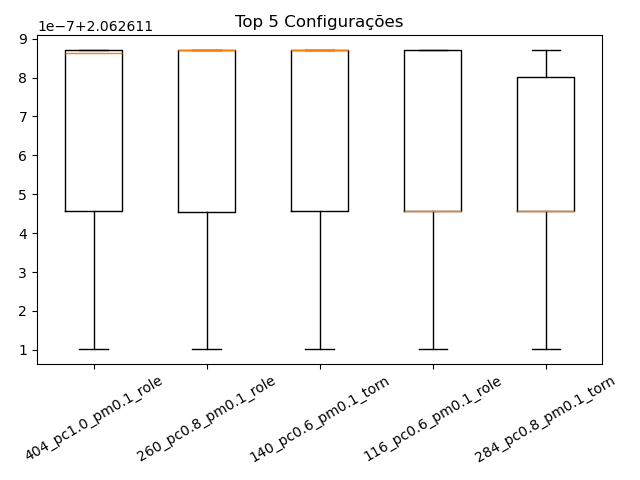
\includegraphics[width=0.90\textwidth]{comparativo_top5.png}
\caption{Boxplot comparativo entre as cinco melhores configurações encontradas.}
\end{figure}

O boxplot das melhores configurações mostra que os resultados de topo apresentaram baixa dispersão, o que reforça a consistência das combinações mais bem-sucedidas.

\subsection{Impacto da Probabilidade de Cruzamento}

\begin{figure}[H]
\centering

\includegraphics[width=0.80\textwidth]{boxplot_pc.png}
\caption{Distribuição dos resultados para diferentes probabilidades de cruzamento.}
\end{figure}

\subsection{Impacto da Probabilidade de Mutação}

\begin{figure}[H]
\centering

\includegraphics[width=0.80\textwidth]{boxplot_pm.png}
\caption{Distribuição dos resultados para diferentes probabilidades de mutação.}
\end{figure}

\subsection{Impacto do Método de Seleção}

\begin{figure}[H]
\centering

\includegraphics[width=0.80\textwidth]{boxplot_selecao.png}
\caption{Distribuição dos resultados para os métodos de seleção utilizados.}
\end{figure}

\subsection{Impacto do Tamanho da População}

\begin{figure}[H]
\centering

\includegraphics[width=0.80\textwidth]{boxplot_populacao.png}
\caption{Distribuição dos resultados para diferentes tamanhos de população.}
\end{figure}

\subsection{Impacto do Número de Gerações}

\begin{figure}[H]
\centering

\includegraphics[width=0.80\textwidth]{boxplot_geracoes.png}
\caption{Distribuição dos resultados para diferentes números de gerações.}
\end{figure}

\subsection{Impacto do Elitismo}

\begin{figure}[H]
\centering

\includegraphics[width=0.80\textwidth]{boxplot_elitismo.png}
\caption{Distribuição dos resultados com e sem elitismo.}
\end{figure}

\subsection{Gráfico de Convergência}

\begin{figure}[H]
\centering
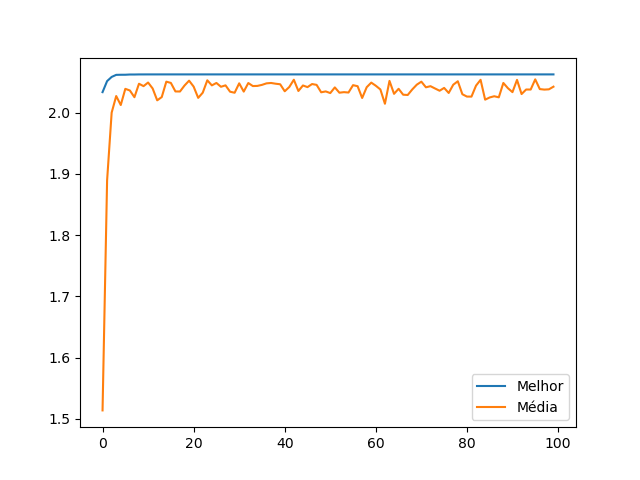
\includegraphics[width=0.90\textwidth]{convergencia_melhor.png}
\caption{Evolução da fitness média e do melhor indivíduo para a melhor configuração encontrada.}
\end{figure}

O gráfico de convergência evidencia que a população evolui progressivamente para regiões de melhor qualidade, com crescimento da fitness média e aproximação do melhor indivíduo ao ótimo encontrado.

%====================================================
% ANÁLISE DOS RESULTADOS
%====================================================

\section{Análise dos Resultados}

Os resultados mostraram que o desempenho do Algoritmo Genético depende fortemente da configuração de seus parâmetros.

Em relação à probabilidade de mutação, observou-se que as melhores configurações utilizaram majoritariamente o valor $pm = 0.1$, correspondente à maior taxa testada. Isso sugere que, para as funções escolhidas neste trabalho, uma capacidade maior de exploração foi importante para evitar aprisionamento em ótimos locais, especialmente no caso da função Cross-in-Tray.

Quanto à probabilidade de cruzamento, verificou-se que valores elevados se destacaram entre as melhores configurações, com $pc = 1.0$ presente na melhor combinação global. Esse comportamento indica que a recombinação intensa entre indivíduos favoreceu a formação de novas soluções promissoras.

No que diz respeito ao método de seleção, tanto roleta quanto torneio apresentaram bons resultados em diferentes cenários. Entretanto, a melhor configuração global utilizou roleta. Isso indica que, quando associada a elitismo, população elevada e mutação intensa, a seleção por roleta foi bastante competitiva.

O tamanho da população apresentou impacto bastante evidente. As configurações com população 100 dominaram grande parte das melhores posições observadas, sugerindo que a maior diversidade genética fornecida por populações maiores contribuiu para a qualidade final das soluções.

Da mesma forma, o número de gerações influenciou diretamente o desempenho. As melhores configurações concentraram-se em 100 gerações, mostrando que o algoritmo se beneficiou de maior tempo evolutivo para refinamento das soluções.

O elitismo também apresentou contribuição relevante. As execuções com elitismo ativado mostraram maior estabilidade, menor dispersão e menor risco de perda dos melhores indivíduos entre gerações, o que favoreceu a convergência.

Na comparação entre as funções objetivo, a função Cross-in-Tray mostrou-se mais desafiadora, por possuir elevada multimodalidade e grande quantidade de ótimos locais. Já a função Drop-Wave apresentou comportamento mais regular e convergência relativamente mais previsível.

Do ponto de vista de implementação, também foi importante corrigir um problema na seleção por roleta, causado pelo uso de fitness negativos. A normalização desses valores foi essencial para garantir a validade da seleção probabilística e a consistência experimental do trabalho.

%====================================================
% CONCLUSÃO
%====================================================

\section{Conclusão}

O Algoritmo Genético implementado mostrou-se eficaz para a resolução de problemas de otimização com duas variáveis, atendendo aos requisitos propostos na atividade.

A utilização de representação binária, operadores genéticos clássicos e análise experimental com múltiplas configurações permitiu não apenas implementar o algoritmo, mas também compreender com maior profundidade a influência dos parâmetros no seu desempenho.

Os resultados indicaram que configurações com maior população, maior número de gerações, elitismo ativado e maior taxa de mutação foram particularmente eficazes nos problemas considerados.

Além de cumprir o objetivo da atividade, este trabalho também estabeleceu uma base reutilizável para experimentos futuros com outros algoritmos evolutivos, como PSO e ACO, ao longo da disciplina.

%====================================================
% REPOSITÓRIO
%====================================================

\section{Repositório do Código}

O código-fonte completo utilizado neste trabalho encontra-se disponível no repositório GitHub:

\begin{center}
\url{https://github.com/higinomatheus/implementacoes_computacao_evolucionaria/tree/main/rel_01_ag}
\end{center}

%====================================================
% REFERÊNCIAS
%====================================================

\bibliographystyle{plainnat}
\bibliography{referencias}

\end{document}